\chapter{Ontwerp van de oplossing en de benodigde onderdelen}
\label{Ontwerp_van_de_oplossing_en_de_benodigde_onderdelen}
%%%%%%%%%%%%%%%%%%%%%%%%%%%%%%%%%%%%%%%%%%%%%%%%%%%%%%%%%%%%%%%%%%%%%%%%

%%%%%%%%%%%%%%%%%%%%%%%%%%%%%%%%%%%%%%%%%%%%%%%%%%%%%%%%%%%%%%%%%%%%%%%%
\section{Hardware}
%%%%%%%%%%%%%%%%%%%%%%%%%%%%%%%%%%%%%%%%%%%%%%%%%%%%%%%%%%%%%%%%%%%%%%%%

het mechanich ontwerp van de printer was grotendeels al gedaan, echter zijn er een aantal aanpassingen gedaan, die staan hier beschreven

%%%%%%%%%%%%%%%%%%%%%%%%%%%%%%%%%%%%%%%%%%%%%%%%%%%%%%%%%%%%%%%%%%%%%%%%
\subsection{Ge-3D-printe oplossingen}
%%%%%%%%%%%%%%%%%%%%%%%%%%%%%%%%%%%%%%%%%%%%%%%%%%%%%%%%%%%%%%%%%%%%%%%%

Een aantal problemen zijn opgelost door kleine onderdelen te 3d printen. hier zijn
daar een paar voorbeelden van.

%%%%%%%%%%%%%%%%%%%%%%%%%%%%%%%%%%%%%%%%%%%%%%%%%%%%%%%%%%%%%%%%%%%%%%%%
\subsubsection{Voetjes van de printer}
%%%%%%%%%%%%%%%%%%%%%%%%%%%%%%%%%%%%%%%%%%%%%%%%%%%%%%%%%%%%%%%%%%%%%%%%

De voetjes van de printer waren te kort, dus daar zijn langere voor
ontworpen en ge-3D-print. Zie Figuur ~\ref{fig:voetjes} voor een render van
het \ac{3d} ontwerp.

\begin{figure}[h]
    \centerline{
\includegraphics[width=0.45\textwidth]{voetjes}}
    \caption{Render van het \ac{3d} ontwerp van de voetjes van de printer}
    \label{fig:voetjes}
\end{figure}

%%%%%%%%%%%%%%%%%%%%%%%%%%%%%%%%%%%%%%%%%%%%%%%%%%%%%%%%%%%%%%%%%%%%%%%%
\subsubsection{Afstandhouder}
%%%%%%%%%%%%%%%%%%%%%%%%%%%%%%%%%%%%%%%%%%%%%%%%%%%%%%%%%%%%%%%%%%%%%%%%

De originele printer is omgebouwd met roestvrijstalen panelen aan alle kanten.
Om ervoor te zorgen dat er goede thermische isolatie is van de print kamer, is
het een dubbelwandig ontwerp met glaswol er tussen. De dubbele wanden worden op
afstand gehouden met ge-3D-printe afstandhouders. Zie Figuur
~\ref{fig:afstandhouder} voor een render van het \ac{3d} ontwerp van deze
afstandhouders.

%%%%%%%%%%%%%%%%%%%%%%%%%%%%%%%%%%%%%%%%%%%%%%%%%%%%%%%%%%%%%%%%%%%%%%%%
\subsubsection{Haakje}
%%%%%%%%%%%%%%%%%%%%%%%%%%%%%%%%%%%%%%%%%%%%%%%%%%%%%%%%%%%%%%%%%%%%%%%%

Om de deur dicht te houden is er een haakje geprint. Zie Figuur
~\ref{fig:haakje} voor een render van het \ac{3d} ontwerp van het haakje.

\begin{figure}[h]
    \centering
    \begin{minipage}{0.45\textwidth}
        \centerline{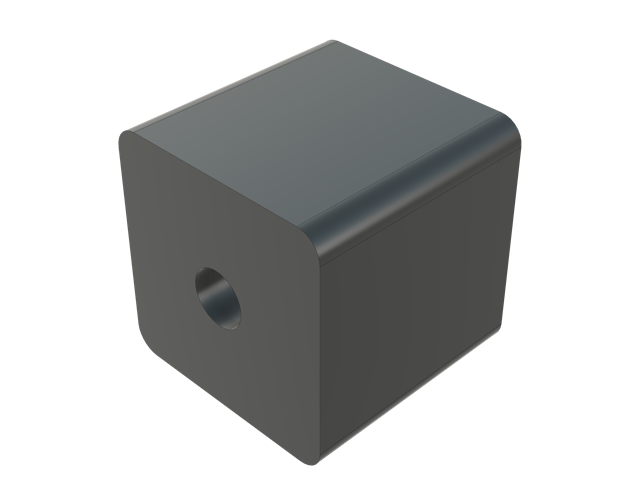
\includegraphics[width=0.9\textwidth]{afstandhouder}}
        \caption{Render van het \ac{3d} ontwerp van de afstandhouder van de printer}
        \label{fig:afstandhouder}
    \end{minipage}\hfill
    \begin{minipage}{0.45\textwidth}
        \centerline{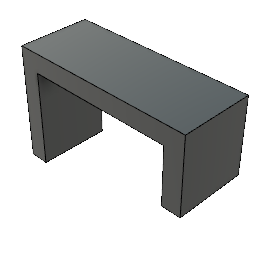
\includegraphics[width=0.9\textwidth]{haakje}}
        \caption{Render van het \ac{3d} ontwerp van het haakje van de printer}
        \label{fig:haakje}
    \end{minipage}
\end{figure}

%%%%%%%%%%%%%%%%%%%%%%%%%%%%%%%%%%%%%%%%%%%%%%%%%%%%%%%%%%%%%%%%%%%%%%%%
\section{Electronica}
%%%%%%%%%%%%%%%%%%%%%%%%%%%%%%%%%%%%%%%%%%%%%%%%%%%%%%%%%%%%%%%%%%%%%%%%

De te gebruiken electronica was grootendeels al vastgesteld voor het project begon.

%%%%%%%%%%%%%%%%%%%%%%%%%%%%%%%%%%%%%%%%%%%%%%%%%%%%%%%%%%%%%%%%%%%%%%%%
\section{Software}
%%%%%%%%%%%%%%%%%%%%%%%%%%%%%%%%%%%%%%%%%%%%%%%%%%%%%%%%%%%%%%%%%%%%%%%%

%%%%%%%%%%%%%%%%%%%%%%%%%%%%%%%%%%%%%%%%%%%%%%%%%%%%%%%%%%%%%%%%%%%%%%%%
\section{Firmware}
%%%%%%%%%%%%%%%%%%%%%%%%%%%%%%%%%%%%%%%%%%%%%%%%%%%%%%%%%%%%%%%%%%%%%%%%

%%%%%%%%%%%%%%%%%%%%%%%%%%%%%%%%%%%%%%%%%%%%%%%%%%%%%%%%%%%%%%%%%%%%%%%%
% \subsection{Subsection}
%%%%%%%%%%%%%%%%%%%%%%%%%%%%%%%%%%%%%%%%%%%%%%%%%%%%%%%%%%%%%%%%%%%%%%%%

